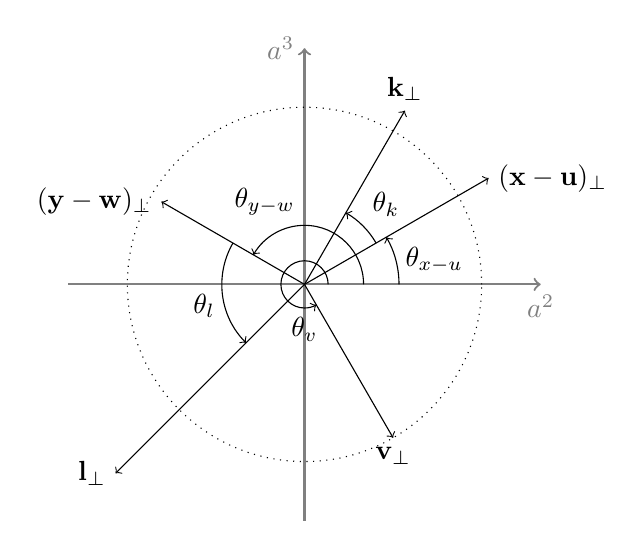
\begin{tikzpicture}[scale=1.5]
%axes
\draw[->,gray,thick] (-2,0) -- (2,0) node[below] {$a^2$};
\draw[->,gray,thick] (0,-2) -- (0,2) node[left] {$a^3$}; 
%circle
\draw[color = black,dotted] (0,0) circle (1.5);
%vectors
\draw[->] (0,0) -- (1.559,0.9) node[right] {$(\mathbf{x}-\mathbf{u})_\perp$};
\draw[->] (0,0) -- (0.85,1.472) node[above] {$\mathbf{k}_\perp$};
\draw[->] (0,0) -- (-1.212,0.7) node[left] {$(\mathbf{y}-\mathbf{w})_\perp$};
\draw[->] (0,0) -- (-1.6,-1.6) node[left] {$\mathbf{l}_\perp$};
\draw[->] (0,0) -- (0.75,-1.299) node[below] {$\mathbf{v}_\perp$};

%arcs
\draw[->] (0.8,0) arc [start angle=0, end angle=30, radius=0.8] node[pos=0.5, right] {$\theta_{x-u}$};
\draw[->] (0.5,0) arc [start angle=0, end angle=150, radius=0.5] node[pos=0.6, above left] {$\theta_{y-w}$};
\draw[->] (0.2,0) arc [start angle=0, end angle=300, radius=0.2] node[pos=0.9, below] {$\theta_v$};
\draw[->] (0.606,0.35) arc [start angle=30, end angle=60, radius=0.7] node[pos=0.5, above right] {$\theta_k$};
%\node at (0.7,0.7) {$\theta_k$};
\draw[->] (-0.606,0.35) arc [start angle=150, end angle=225, radius=0.7] node[pos=0.6, left] {$\theta_l$};
%\node at (-0.7,-0.2) {$\theta_l$};
\end{tikzpicture}